%NOTE!  Do NOT change anything in this section!
\documentclass[11pt]{article} 
\usepackage{graphicx}
\usepackage{geometry}               
\geometry{letterpaper}
\geometry{portrait}
\usepackage{multicol}
\usepackage{hyperref}
\usepackage[parfill]{parskip} 
\usepackage{times}
\usepackage{wrapfig}
\usepackage[utf8]{inputenc}
\usepackage[english]{babel}
\usepackage{booktabs}
\usepackage{listings}
\usepackage{mathtools}
\usepackage{multirow}
\lstset{basicstyle=\small\ttfamily}

\begin{document}
%  NOW you can start changing stuff!

\title{A Computational Approach to Predict Chances of Survival in Myocardial Infarction Patients Using Echocardiogram Measurements
\thanks{
Correspondence to:  sudhir20k@ncssm.edu}
}


\author{Krishna Sudhir\\
{\it NCSSM Online}\\
{\it  North Carolina School of Science and Mathematics}\\
{\it Durham, North Carolina}\\
 }
\date{15 January, 2019}

\maketitle  % don't touch this!


\begin{quotation}
\textbf{Abstract:}  Echocardiograms are one of the medical imaging techniques that use high frequency sound waves (ultrasound) to take pictures of the heart. Victims of heart attacks are posed with a significant risk of mortality within one year of their heart attack. Having foresight into their patients' chance of survival would enhance the ability of medical professionals in forming accurate prognosis and prescribing effective medical interventions. This research project aims to develop a computational model that will predict patients’ chances of survival by using statistical modeling using attributes derived from various measurements from echocardiograms. This model would utilize a number of potentially significant predictor attributes to predict one binary dependent variable, which is the chance of survival at least for a year given the measurements of the predictor variables. The main statistical method employed was a logistic regression model. The model accuracy has been measured by a number of cross validation methods. The final model was found to be quite reliably predictive of the outcome when tested with the test data. The attributes found to be significant in this final model were age, fractional shortening and wallmotion-index measurements. This promises scope for future expansive study and in turn could lead to building health care applications that could leverage such computational models. \\


\textbf{Key words:} Echocardiogram, Myocardial Infarction, Logistic Regression, Health Data, Wallmotion Index, R, Computational Sciences, Statistics, Modeling, Cardiology

\end{quotation}

\newpage
{\bf Introduction}

A comprehensive study had been conducted from June 1981 to June 1983 by the department of Cardiology in the University of Amsterdam to understand the predictive ability of wall motion score of patients  of their cardiac health \cite{gerard}. Speckle-tracking echocardiography (STE) allows to calculate wall motion score index, which has been utilized as a surrogate to determine patients’ myocardial health \cite{nesser}. It is a measure of how the segments of the left ventricle are moving. In this study, the wall motion score index along with many other indices were calculated at the time of admission and the patients were tracked for another year for any cardiac events. The correlation between wall motion scores and the occurrences of cardiac events has been empirically established for having significant capability for predicting future events. 

It was recorded that about 20\% of the 345 patients participating in the study had died within only one year following heart attack \cite{gerard}. Given such high probability of mortality, it is imperative that predictive mechanisms are accessible to doctors in order to effectively treat and monitor patients after cardiac events. Mortality rate varies significantly between patients and is dependent on present and previous health, environmental factors and future lifestyle. This makes chances of survival really hard to predict accurately. 

Cross sectional echocardiography allows for a three dimensional view of heart functionality by use of two- dimensional cross sections of echocardiography through ultrasound waves. Echocardiography is a noninvasive and safe method of visualization, without involving breaking of the skin or risk for side effects. Echocardiograms not only track heart functionality but report back data indicating size, shape, and presence of tissue damage \cite{echo}. Figure \ref{fig:SampleEchocardiogram} shows a typical echocardiogram.

%\end{multicols}
\begin{figure}[htbp]
\centering
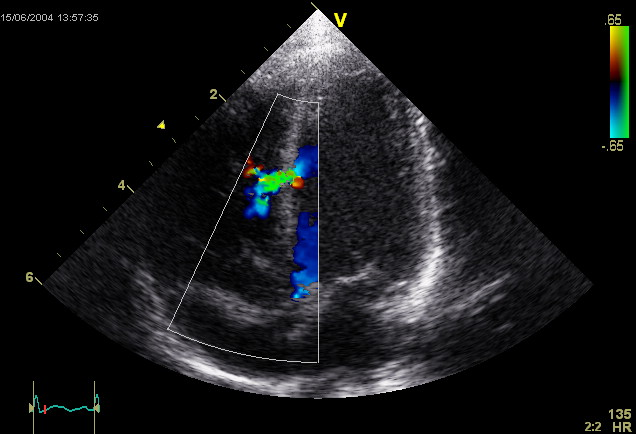
\includegraphics[scale=0.5]{Ventricular_Septal_Defect.jpg}
\caption{A typical Echocardiogram showing ventricular septal defect \cite{echo}}
\label{fig:SampleEchocardiogram}
\end{figure}
%\begin{multicols}{2}

{\textbf {\emph{Data Description}}}

This study has been conducted on a specific dataset hosted by University of California Irvine (UCI) \cite{data}. The dataset is relatively small with observations from 131 individuals. Listing \ref{DataSummary} shows a summary of the dataset, with statistical distributions and the counts of missing data. It has numerous instances with missing values. However small it might be, the data promises good insight into how the easy-to-measure attributes could be leveraged to predict the survival rate with reasonable accuracy. Table \ref{table:DataAttributes} shows the data attributes and their descriptions.

%\end{multicols}



\begin{lstlisting}[label=DataSummary, caption=Summary of Data, float, frame=tb]

    survival          alive             age       
 Min.   : 0.030   Min.   :0.0000   Min.   :35.00  
 1st Qu.: 7.875   1st Qu.:0.0000   1st Qu.:57.00  
 Median :23.500   Median :0.0000   Median :62.00  
 Mean   :22.183   Mean   :0.3282   Mean   :62.81  
 3rd Qu.:33.000   3rd Qu.:1.0000   3rd Qu.:67.75  
 Max.   :57.000   Max.   :1.0000   Max.   :86.00  
 NA's   :3        NA's   :2        NA's   :7   

 pericardialeffusion fractionalshortening      epss      
 Min.   : 0.0000     Min.   :0.0100       Min.   : 0.00  
 1st Qu.: 0.0000     1st Qu.:0.1500       1st Qu.: 7.00  
 Median : 0.0000     Median :0.2050       Median :11.00  
 Mean   : 0.7651     Mean   :0.2167       Mean   :12.16  
 3rd Qu.: 0.0000     3rd Qu.:0.2700       3rd Qu.:16.10  
 Max.   :77.0000     Max.   :0.6100       Max.   :40.00  
 NA's   :1           NA's   :9            NA's   :16   
 
      lvdd       wallmotion.score wallmotion.index      mult       
 Min.   :2.320   Min.   : 2.00    Min.   :1.000    Min.   :0.1400  
 1st Qu.:4.230   1st Qu.:11.00    1st Qu.:1.000    1st Qu.:0.7140  
 Median :4.650   Median :14.00    Median :1.216    Median :0.7860  
 Mean   :4.763   Mean   :14.44    Mean   :1.378    Mean   :0.7862  
 3rd Qu.:5.300   3rd Qu.:16.50    3rd Qu.:1.508    3rd Qu.:0.8570  
 Max.   :6.780   Max.   :39.00    Max.   :3.000    Max.   :2.0000  
 NA's   :12      NA's   :5        NA's   :3        NA's   :4       


   name      group       aliveat1     
     :  1       : 1   Min.   :0.0000  
 name:131   1   :24   1st Qu.:0.0000  
 NA's:  1   2   :85   Median :0.0000  
            name: 1   Mean   :0.3333  
            NA's:22   3rd Qu.:1.0000  
                      Max.   :1.0000  
                      NA's   :58     

\end{lstlisting}




\begin{table}[htbp]
\centering
\begin{tabular}{@{}ll@{}}
Attribute             & Description                                                                                                                                                                                                                         \\ \hline
Survival              & Number of months patient has survived after heartattack.                                                                                                                                                                            \\ \hline
Age                   & Age at which heart attack occurred                                                                                                                                                                                                  \\ \hline
Pericardial effusion  & \begin{tabular}[c]{@{}l@{}}Binary variable, whether or not fluid is present around heart.\\    0 = no fluid present\\    1 = fluid present around heart\end{tabular}                                                                \\ \hline
Fractional shortening & A measure of the contractility around the heart. Lower numbers are abnormal.                                                                                                                                                        \\ \hline
epss                  & \begin{tabular}[c]{@{}l@{}}Another measure of contractility.\\ Larger numbers are abnormal.\\ E-point septal separation {[}4{]}\end{tabular}                                                                                        \\ \hline
lvdd                  & \begin{tabular}[c]{@{}l@{}}Stands for left ventricular end-diastolic dimension. \\ Lvdd is a measure of the size of the heart at end-diastole. \\ Larger number indicates that those hearts tend to have more issues.\end{tabular}  \\ \hline
wallmotion-score      & A measure of how the segments of the left ventricle are moving                                                                                                                                                                      \\ \hline
wallmotion-index      & \begin{tabular}[c]{@{}l@{}}Can be derived by dividing wallmotion-score by number of segments observed. \\ Usually 12-13 segments are seen in an echocardiogram. \\ This variable was used instead of wallmotion-score.\end{tabular} \\ \hline
aliveat1              & \begin{tabular}[c]{@{}l@{}}Whether or not patient is alive after 1 year.\\     0 = dead after 1 year \\     1 = alive after 1 year (boolean variable)\end{tabular}                                                           \\ \hline      
\end{tabular}
\caption{Data attributed and description}
\label{table:DataAttributes}
\end{table}

%\begin{multicols}{2}

{\bf Computational Approach}

The dataset contained echocardiogram measurements from 133 individuals whose survival rate was tracked for more than a year. Even though the data has interesting information, there were some outlier values and many more missing values. This posed a difficult challenge to build, train and test the model. To address this, a comprehensive data cleanup was attempted. Figure \ref{fig:Histogram} shows the histograms of all the important predictor variables.

%\end{multicols}
\begin{figure}[htbp]
\centering
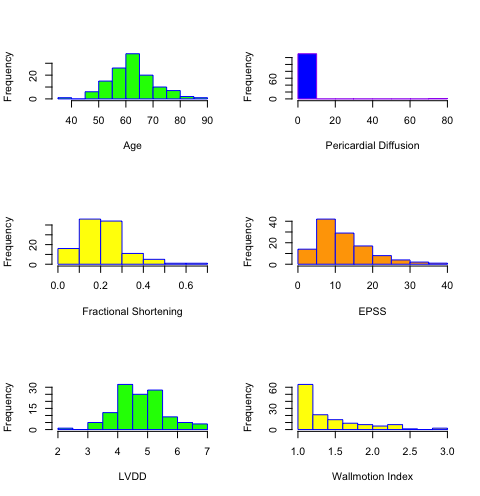
\includegraphics[scale=0.75]{Histogram.png}
\caption{Histogram distribution of predictor variables}
\label{fig:Histogram}
\end{figure}

%\begin{multicols}{2}

{\textbf {\emph{Handling of Outliers}}}

Outliers were removed or capped. For example, one of the individuals had aliveat1 value of 2 instead of the acceptable value of 0 or 1. This was capped at 1. 

{\textbf {\emph{Handling of Missing Values}}}

There were quite a few observations with missing values. These observations have to be either filled in or removed in order to have a reliable predictive model. If there were missing values for the dependent variable (aliveat1), those rows were not considered in the model. Other missing values were a) removed, b) replaced with a mean value or c) replaced with a median value. The model with all missing values removed was considered to be the benchmark. The accuracy of each approach was compared against the benchmark accuracy. The listing \ref{DataCleanup} shows snippets of these strategies.


\begin{lstlisting}[language=R, label=DataCleanup, caption=Data Cleanup Methods, float, frame=tb]
#
# Replace the missing value with the median
echoData$age[is.na(echoData$age)] <- median(echoData$age,na.rm=T)

#
# Replace the missing value with the mean
echoData$age[is.na(echoData$age)] <- mean(echoData$age,na.rm=T)

#
# Remove all rows with missing values
cleanEcho <- na.omit(echoData)
\end{lstlisting}



{\textbf {\emph{Training and Test Data}}}

The dataset was divided into a test set and training set. 75\% of the records were used to train the model and 25\% of the records was used for testing the model for prediction accuracy.


{\textbf {\emph{The Model}}}

Since the dependent variable was a boolean variable (aliveat1 is either 1 or 0, representing whether the individual was alive after that year or not, respectively), a logistic regression approach was considered for modeling. A binary logistic regression is a method used to model data with a dichotomous dependent variable, or a binary outcome. Logistic regressions can be derived from the equation \ref{eqn:logit}:

\begin{equation}
\label{eqn:logit}
    \ln(\frac{p}{(1-p)}) = a + \beta * X + e
\end{equation}

There are 12 candidate variables to be examined to determine which of them are potentially significant. Data visualization showed that the fields do not show explicit patterns. Some of the attributes have the same value for all the observations. Those observations were visually identified and removed from the model. The rest of the variables were considered significant for the study and were further analyzed by univariate logistic regression on each one of those variables. By comparing the p value and accuracy, the influence of the individual variables were compared. 

In the next step, a multivariate logistic regression model with all the significant variables was tried out for accuracy. From this model, individual variables were removed to see if the prediction accuracy improved. Through an iterative process, a multivariate model was devised.


The 'stat' library of R provides out of the box functions to run logistic regression as well as predict outcomes based on the model created. The function 'glm' (Generalized Linear Model) with an option to use binomial method, would conveniently return the logistic model. Using this facility, a multivariate logistic regression was carried out with “aliveat1” as the dependent variable and the following variables - age, pericardial effusion, fractionalshortening, wallmotion.index, lvdd, and epss as the predictors.


The 'predict' method of the stat library returns the predicted values. By comparing the predicted outcomes with the actual outcomes in the test dataset, one can determine the accuracy of the model.  The listing \ref{LogisticModel} shows the model building and validation methodology. In the final model, it was determined that the only significant predictor variables are age, wallmotion.index and fractionalshortning.

{\it The p Value}

The 'p' values were analyzed for each of the predictor variables to evaluate their significance. The 'p' values were reported to have higher values than expected. Therefore, additional methods to compare the accuracy were employed.

{\textbf {\emph{Model Benchmarking}}}

There were a number of methods to compare the accuracy of the models with one another. Using Accuracy, RMSE (Root Mean Square Error), Concordance vs Discordance ratio, misclassfication error, confusion matrix, Specificity vs Sensitivity, ROC curve and KS Plot the models were compared and classified based on their performance. Each of these methods helped in determination of the better model \cite{errormetrics}.

{\it Accuracy}

Prediction error was calculated by taking the mean of all the differences between predicted outcomes and actual outcomes. Accuracy was measured using Equation \ref{eqn:AccuracyEqn}

\begin{equation}
\label{eqn:AccuracyEqn}
    PredictionAccuracy = 1 - PredictionError
\end{equation}

{\it RMSE}

RMSE is a measure of how accurate the model is by squaring the differences of predictions and actuals and then taking the square root of their average. Lower the RMSE the better the model is. The equation \ref{eqn:RMSE} shows how to calculate RMSE. 

\begin{equation}
\label{eqn:RMSE}
RMSE = \sqrt{\frac{1}{n}\Sigma_{i=1}^{n}{\Big(\frac{d_i -f_i}{\sigma_i}\Big)^2}}
\end{equation}

{\it Confusion Matrix}

Confusion matrix gives a useful but simple interpretation of the model's accuracy. It gives a grid of true positives, false positives, true negatives and false negatives. This gives an idea where the model performs well and where it doesn't. From the library {\it InformationValue} the function {\it confusionMatrix()} was used to calculate the Confusion Matrix of the models that were studied.

{\it Kolmogorov-Smirnov Plot}

Kolmogorov-Smirnov test can be used for determining the performance of classification models. It tests the degree of separation between the positive and negative distributions in the models predicted output. From the library {\it InformationValue} the function {\it ks\_plot()} was used to plot the results of K-S chart.


{\textbf {\emph{Validation Methodology}}}

Since the dataset was small and had many records missing values, the models were susceptible to either overfitting or underfitting. The test set used for model validation seemed to be small to evaluate the model reliably. Multiple validation methods were utilized to address this deficiency.

{\it 1. Train / Test Data Split}

In order to build a training model to test the accuracy of the model, the data was partitioned into two groups, training and testing sets, with 75 percent of the data and 25 percent of the data respectively. Using the training data to build the model, the testing data is run through the model in order to ensure accuracy above 50\%. While splitting of the data into 75\% and 25\% is the most convenient and computationally least expensive, especially for larger data sets, when it comes to smaller, unreliable datasets, such a split may very well lead to overfitting and/or underfitting.

Overfitting of data is a modeling error where the model is too closely related to the data used to train the model. While the model will be very close to the data, it will be very prone to error when predicting outcomes while testing. Overfitting occurs when there is too little data for researchers to train and create the model, or when the data used to train the model has an excess of outliers. Overfitted models will exhibit low bias, which is the difference between the expected output of the model and the true outcome. A model with a high bias will be too specific to the training data and values predicted for the model from the  training set will vary little with the true outcome \cite{bias-variance}. The model will be highly accurate but will exhibit very little predictive ability due to high variance. Variance is the extent at which predicted values of the model vary with the true outcome of future outcomes. 

{\it 2. Leave One Out Cross Validation (LOOCV)}

Cross validation is a method by which the model can be evaluated based upon its ability to predict new outcomes of data that it has not been exposed to before. By splitting the data into training and testing groups, and building the model with the training group, the model is only accustomed to one training group and one testing group. Cross validation allows for the  building of the model with more data to reduce chances of overfitting and the high variance and low bias because of such.

“Leave-one-out” cross validation is done by using only one instance to test the model, and the rest of the data to train the model. While this creates a model that is not overfitted, and has low bias, there are two major drawbacks to LOOCV. This type of cross validation will repeat the training a multitude of times with a significantly higher amount of data which will reduce chances of overfitting. There will be very high variability in the model since only one instance was used for prediction. Additionally, due to there only being one instance being used for prediction, the model will be trained through multiple iterations and for large data sets, this type of cross validation can be computationally expensive \cite{k-fold}.

{\it 3. K-Fold Cross Validation}

The model will be trained using every data set “k-1” times and this type of cross validation allows the user to independently choose how large each testing set is and how many times the model will run \cite{k-fold}. While this type of cross validation can also be computationally expensive when dealing with large datasets, it is a reasonable middle ground between LOOCV and normal evaluation \cite{crossval} 

One of the additional computational tasks in K-Fold Cross Validation is to iteratively find an optimal value for {\it k}. For values of {\it k} between two and twelve, the model was run to get an optimum k value by comparing the predictive error and the adjusted predictive error to find the lowest value. This value can be used in the final model that was selected. {\it cv.glm} function from {\it boot} library was used for K-fold cross validation.

\newpage
{\bf Results and Discussion}

One of the major drawbacks of the data was the relatively  large amount of missing values and its small number of observations. Removing the missing values seemed to be working well for accuracy. 

{\it Multicollinearity}

All the predictor variables were used in a test model to calculate the VIF matrix as shown in Table \ref{table:VIFScores}. This method showed there was little multicollinearity (dependency between the predictor variables). The VIF score for all variables were under 2, which indicates that there is little collinearity between the fields \cite{vif}. 

\begin{table}[htbp]
\centering
\begin{tabular}{@{}lc@{}}
\toprule
\textbf{Field name}  & \multicolumn{1}{l}{\textbf{Variable Inflation Factor (VIF)}} \\ \midrule
Age                  & 1.219                                                        \\
Pericardialeffusion  & 1.365                                                        \\
Fractionalshortening & 1.387                                                        \\
Wallmotion.index     & 1.412                                                        \\
Lvdd                 & 1.413                                                        \\
Epss                 & 1.948                                                        \\ \bottomrule
\end{tabular}
\caption{Variable Inflation Factor for the Attributes}
\label{table:VIFScores}
\end{table}

{\it Model Performance}

A number of univariate and multivariate models were attempted using logistic regression and their accuracy was benchmarked. Table \ref{table:ModelParams} shows all the models that were used for this study. 

\begin{table}[htbp]
\centering
\begin{tabular}{@{}lll@{}}
\toprule
\textbf{Model \#} & \textbf{Model name} & \textbf{Model equation}                                                                    \\ \midrule
1                 & Model-01            & aliveat1 $\sim$age                                                                         \\
2                 & Model-02            & aliveat1 $\sim$pericardialeffusion                                                         \\
3                 & Model-03            & aliveat1 $\sim$fractionalshortening                                                        \\
4                 & Model-04            & aliveat1 $\sim$wallmotion.index                                                            \\
5                 & Model-05            & aliveat1 $\sim$wallmotion.score                                                            \\
6                 & Model-06            & aliveat1 $\sim$lvdd                                                                        \\
7                 & Model-07            & aliveat1 $\sim$epss                                                                        \\
8                 & Model-08            & aliveat1 $\sim$age + fractionalshortening + wallmotion.index                               \\
9                 & Model-09            & aliveat1 $\sim$age + fractionalshortening + wallmotion.score                               \\
10                & Model-10            & aliveat1 $\sim$age + fractionalshortening + wallmotion.index + lvdd                        \\
11                & Model-11            & aliveat1 $\sim$age + fractionalshortening + wallmotion.index + lvdd + epss                 \\
12                & Model-12            & aliveat1 $\sim$age + fractionalshortening + wallmotion.index + epss                        \\
13                & Model-13            & aliveat1 $\sim$fractionalshortening + wallmotion.index + epss + lvdd                       \\
14                & Model-14            & aliveat1 $\sim$fractionalshortening + wallmotion.index + epss + lvdd + pericardialeffusion \\ \bottomrule
\end{tabular}
\caption{Univariate and Multivariate Models and Parameters}
\label{table:ModelParams}
\end{table}


The table \ref{table:RegressionResults} show the various accuracy measurements such as AIC, RMSE for each of the model. The lowest level of accuracy was 65\% where as the highest scored upto 83\%. Model-08 was selected as the best performing model out of all the models that were analyzed. In otherwords, a patient's age, fractionalshortening and wallmotion.index measurements taken together have a predictive capability of 83\% on the test data. This model also showed lower AIC score, lower RMSE, lower misclassification error as well as lower Residual Deviance. The scatter plots of these measurements show the results graphically. The plot \ref{fig:AICPlot} show AIC and Residual Deviance for each of the models. The plot \ref{fig:AccuracyPlot} shows Accuracy, RMSE and misclassfication errors of each of the models.

\begin{table}[htbp]
\centering
\begin{tabular}{@{}cccccc@{}}
\toprule
\textbf{Model \#} & \textbf{AIC} & \textbf{Accuracy} & \textbf{RMSE} & \textbf{Misclass Error} & \textbf{Residual deviance} \\ \midrule
1                 & 48.98        & 0.74              & 0.43          & 0.26                    & 44.98                      \\
2                 & 50.57        & 0.65              & 0.47          & 0.35                    & 46.57                      \\
3                 & 47.62        & 0.65              & 0.47          & 0.35                    & 43.62                      \\
4                 & 48.10        & 0.74              & 0.40          & 0.26                    & 44.10                      \\
5                 & 46.39        & 0.78              & 0.43          & 0.22                    & 42.39                      \\
6                 & 49.97        & 0.70              & 0.45          & 0.30                    & 45.97                      \\
7                 & 49.39        & 0.65              & 0.45          & 0.35                    & 45.39                      \\
8                 & 48.52        & 0.83              & 0.36          & 0.17                    & 40.52                      \\
9                 & 46.80        & 0.83              & 0.37          & 0.17                    & 38.80                      \\
10                & 50.47        & 0.78              & 0.37          & 0.22                    & 40.47                      \\
11                & 52.38        & 0.78              & 0.37          & 0.22                    & 40.38                      \\
12                & 50.49        & 0.83              & 0.36          & 0.17                    & 40.49                      \\
13                & 52.44        & 0.70              & 0.41          & 0.30                    & 42.44                      \\
14                & 54.21        & 0.70              & 0.41          & 0.30                    & 42.21                      \\ \bottomrule
\end{tabular}
\caption{Univariate and Multivariate Regression Results}
\label{table:RegressionResults}
\end{table}

\begin{figure}[htbp]
\centering
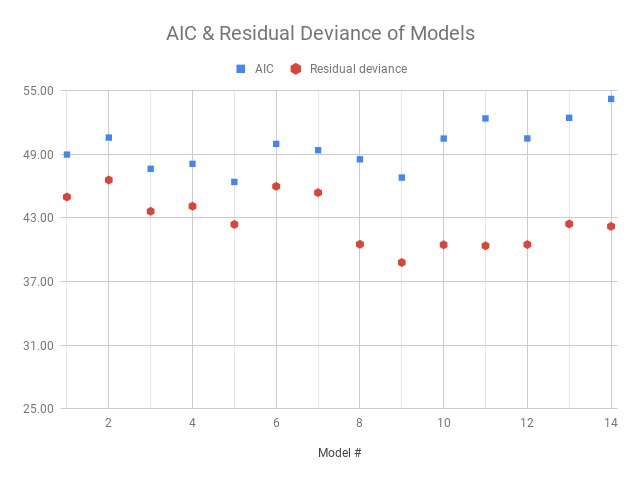
\includegraphics[scale=0.5]{AIC-ResidualDeviance.png}
\caption{AIC and Residual Deviance of Models}
\label{fig:AICPlot}
\end{figure}

\begin{figure}[htbp]
\centering
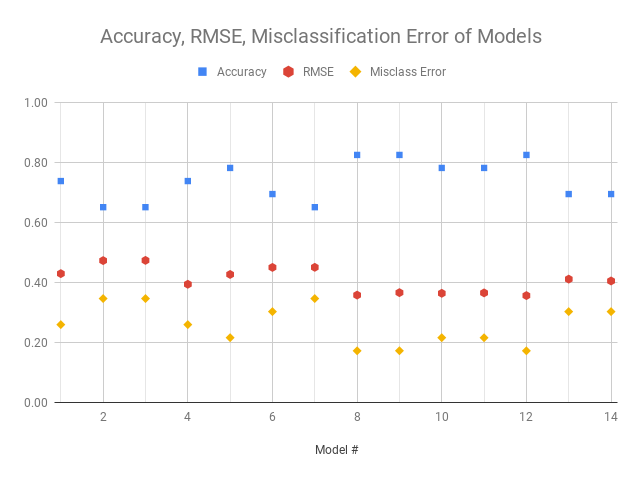
\includegraphics[scale=0.5]{Accuracy-RMSE-MisclassError.png}
\caption{Accuracy, RMSE and Misclassification Error of Models}
\label{fig:AccuracyPlot}
\end{figure}

{\it Confusion Matrix}

Confusion Matrix was calculated and printed for high-performing multivariate models 8, 9 and 12. Table \ref{table:ConfusionMatrix} shows the confusion matrix values. As could be seen, all these models have a tendency to mis-predict false positives. 


\begin{table}[htbp]
\centering
\begin{tabular}{|c|c|c|c|}
\hline
\textbf{Model name}                & \multicolumn{3}{c|}{\textbf{Confusion Matrix}}  \\ \hline
                                   &                & \textit{FALSE} & \textit{TRUE} \\ \hline
\multirow{2}{*}{\textbf{Model-08}} & \textit{FALSE} & 15             & 4             \\ \cline{2-4} 
                                   & \textit{TRUE}  & 0              & 4             \\ \hline
\multirow{2}{*}{\textbf{Model-09}} & \textit{FALSE} & 15             & 4             \\ \cline{2-4} 
                                   & \textit{TRUE}  & 0              & 4             \\ \hline
\multirow{2}{*}{\textbf{Model-12}} & \textit{FALSE} & 15             & 4             \\ \cline{2-4} 
                                   & \textit{TRUE}  & 0              & 4             \\ \hline
\end{tabular}
\caption{Confusion Matrix for Models 8, 9 and 12}
\label{table:ConfusionMatrix}
\end{table}

\newpage
{\it AUROC and Kolmogorov-Smirnov Test}

The selected model was studied further for more benchmarking methods such as plotting ROC curve as well as Kolmogorov–Smirnov plots (KS Plot). ROC curve shows 92.5\% of area under the curve. The ROC Plot (Figure \ref{fig:AUROC}) shows that the model has very good predictive abilities. Additionally the KS Plot (Figure \ref{fig:KSPlot}) shows that the model can predict much higher than the random prediction at the mean level. 

\begin{figure}[htbp]
\centering
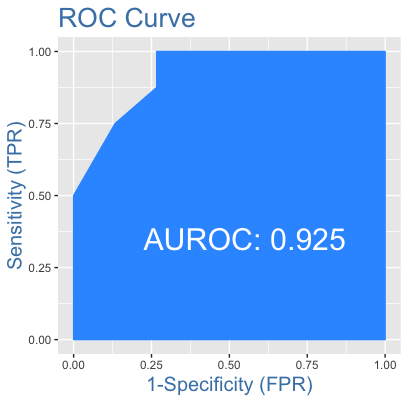
\includegraphics[scale=0.7]{AUROC-08.png}
\caption{AUROC Plot for Model-08}
\label{fig:AUROC}
\end{figure}

\begin{figure}[htbp]
\centering
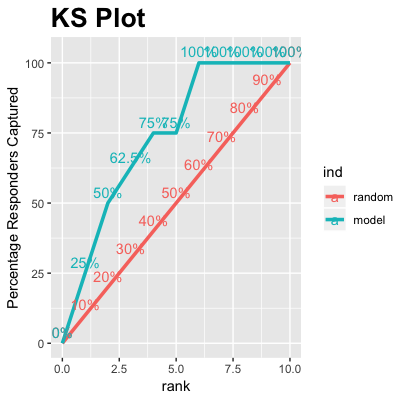
\includegraphics[scale=0.7]{KSPlot-08.png}
\caption{KS Plot of Model-08}
\label{fig:KSPlot}
\end{figure}

{\it Cross Validation Results}

LOOCV method didn't yield better accuracy as predicted. However, K-fold Cross Validation showed comparable performance with Train / Test data split. The optimal value for 'k' was found to be 4 for this dataset as could be seen from Figure \ref{fig:KFold}.

\begin{figure}[htbp]
\centering
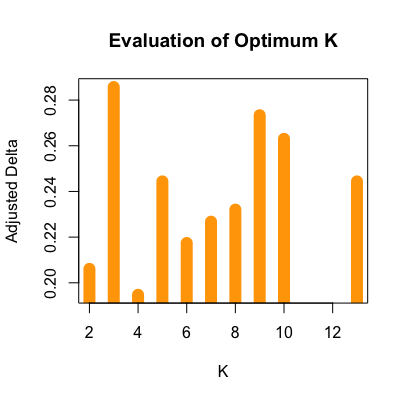
\includegraphics[scale=0.7]{KFoldCV.png}
\caption{Finding K for the K-Fold Cross Validation}
\label{fig:KFold}
\end{figure}

{\it The Final Model}

The final model yielded the coefficients for the predictor variables as given in the Table \ref{table:ModelCoefficients}. If age (a), fractionalshortening (fs) and wallmotion.index(wi) are given, the probability of survival at 1 year for a patient can be determined by the Equation \ref{eqn:LogitEqn}. 

\begin{equation}
\label{eqn:LogitEqn}
\ln(\frac{p}{1 - p}) = 
  -6.07131 
  + 0.07130 * a 
  - 4.69015 * fs 
  + 0.98505 * wi
\end{equation}

\begin{table}[hb]
\centering
\begin{tabular}{@{}ll@{}}
\textbf{}                     & \textbf{Estimate} \\
\textbf{Intercept}            & -6.07131          \\
\textbf{age}                  & 0.07130           \\
\textbf{fractionalshortening} & -4.69015          \\
\textbf{wallmotion.idex}      & 0.98505          
\end{tabular}
\caption{Model Coefficients}
\label{table:ModelCoefficients}
\end{table}

\newpage
{\bf Conclusions}

There were a number of findings from this study that were interesting. A simple model with 3 predictor variables was found to be having very good predictive ability.
\begin{enumerate}
  \item The multivariate model with age, fractional-shortening and wallmotion-index measurements yielded better performance compared to univariate models. The univariate model with wallmotion-score as the predictor had the highest accuracy of all univariate models with 78\% accuracy whereas the multivariate model (Model-08) showed 83\% accuracy.
  \item In practical terms, by using these 3 predictor variables the physicians can adequately determine the probability of survival of a patient for another year after a heart attack and therefore, could plan medical intervention that would improve the chances of survival.
  \item The model accuracy could be improved by having more underlying data for the model to train and evaluate. Collecting more data from physicians would potentially improve the statistical significance of the findings of this study as well.
  \item Further more, the data should be captured from diverse demographics including ethic, economic and gender groups. This would eliminate any data skewness that might limit the model's predictive capabilities.
  \item Logistic regression is one of the widely used methods of modeling and prediction. Other machine learning and deep learning approaches could further improve the predictive accuracy and reliability. Newer algorithms and more cleaner data could assist physicians and other medical professionals to help myocardial patients to live longer.
\end{enumerate}

This analysis only scratched the surface of the untapped potential of hidden data patterns. The power and promise of computational sciences with larger and good quality data could be best utilized for improving human lives.

{\bf Acknowledgements}

The author thanks Mr. Robert Gotwals for giving an opportunity and assistance to work on this interesting problem, as part of the NCSSM coursework, "Introduction to Computational Sciences", which in itself introduced the class a wide variety of tools and practices that immensely helped to conduct this study.  Appreciation is also extended to the NCSSM (North Carolina School of Science and Mathematics) for facilitating various computational sciences courses as part of the curriculum. The author is also grateful to the University of California, Irvine for making this dataset publicly available for the use of researchers.

\newpage
\begin{thebibliography}{5}

\bibitem{gerard}Gerard Kan, Cees A Visser, Jacques J Koolen, Arend J Dunning: "Short and long term predictive value of admission wall motion score in acute myocardial infarction: A cross sectional echocardiographic study of 345 patients" Available at: https://www.ncbi.nlm.nih.gov/pmc/articles/PMC1236887/pdf/brheartj00107-0028.pdf

\bibitem{nesser}Hans Joachim Nesser: “Wall Motion Tracking And Activation Imaging - Latest Developments And Applications For Patients With Heart Failure.” Available at https://www.ecrjournal.com/articles/wall-motion-tracking-and-activation-imaging-latest-developments-and-applications-patients

\bibitem{echo}Echocardiography https://en.wikipedia.org/wiki/Echocardiography 

\bibitem{Elagha}Abdalla Elagha, Anthon Fuisz: “Mitral valve E-Point to Septal Separation (EPSS) measurement by cardiac magnetic resonance Imaging as a quantitative surrogate of Left Ventricular Ejection Fraction (LVEF)” Available at  https://www.ncbi.nlm.nih.gov/pmc/articles/PMC3305188/ 

\bibitem{variance}Variance https://en.wikipedia.org/wiki/Variance

\bibitem{bias}Bias of an estimator "https://en.wikipedia.org/wiki/Bias\_of\_an\_estimator"

\bibitem{bias-variance}Bias-variance tradeoff https://en.wikipedia.org/wiki/Bias-variance\_tradeoff

\bibitem{k-fold}A Gentle Introduction to k-fold Cross Validation https://machinelearningmastery.com/k-fold-cross-validation/

\bibitem{crossval}Cross validation https://www.cs.cmu.edu/~schneide/tut5/node42.html 

\bibitem{logit}An Introduction to Logistic Regression http://www.appstate.edu/~whiteheadjc/service/logit/intro.htm 

\bibitem{errormetrics}7 Important Model Evaluation Error Metrics Everyone should know https://www.analyticsvidhya.com/blog/2016/02/7-important-model-evaluation-error-metrics/

\bibitem{data}University of California Irvine Echocardiogram Dataset: https://archive.ics.uci.edu/ml/datasets/echocardiogram

\bibitem{vif}Multicollinearity: https://en.wikipedia.org/wiki/Multicollinearity

\end{thebibliography}

\newpage
{\bf APPENDIX}
\begin{lstlisting}[language=R, label=LogisticModel, caption=Building Logistic Model and Validating (Snippet), frame=htbp]
set.seed(1234)
model1 <- glm(formula8, family=binomial(), data = echotrain)

prediction1 <- predict(model1, newdata = echotest, type = 'response')
fitted.results <- ifelse(prediction1 > 0.5, 1, 0)

predictionerror <- mean(fitted.results != echotest$aliveat1)
anovaResults <- anova(model1)
score <- rmse(prediction1, echotest$aliveat1)
print("")
print("-------------------------------------------------------")
print(formula8)
print("-------------------------------------------------------")
print(summary(model1))
print(anovaResults)
print(paste("ACCURACY: ", 1-predictionerror))
print(paste("RMSE: ", score))
print("Concordance Analysis:")
print(Concordance(echotest$aliveat1, fitted.results))
print("Misclassification Error Analysis:")
print(misClassError(echotest$aliveat1, fitted.results))
print("Specificity Analysis:")
print(specificity(echotest$aliveat1, fitted.results))
print("Sensitivity Analysis:")
print(sensitivity(echotest$aliveat1, fitted.results))
print("Confusion Matrix:")
print(confusionMatrix(echotest$aliveat1, fitted.results))
sensMatrix <- plotROC(echotest$aliveat1, prediction1, 
      Show.labels = F, returnSensitivityMat = T)
ks_plot(echotest$aliveat1, prediction1)

\end{lstlisting}


\end{document}
